\section{Theory}
\subsection{Reference potential energy}
A measurement of spurious mixing with a physical basis comes from the reference potential energy \citep[known also as background potential energy][]{winters95}. This is the lowest attainable potential energy of a given fluid, where there is no energy available for motion. To calculate this state, the fluid must be adiabatically re-sorted to a stable stratification, where every fluid parcel is spread laterally across the entire domain. The sum of the reference potential energy and the available potential energy (APE) gives the total potential energy in the system. Mathematically, the RPE is expressed as

\begin{equation}
  \mathrm{RPE} = g \int_\Omega z \rho^*(z)\,\mathrm dV,
\end{equation}

where $g$ is the gravitational constant; $z$ is the height, positive upward; $\Omega$ is the domain; $V$ is the volume; and $\rho^*$ is the adiabatically re-sorted density profile, known as the reference density. The reference density is well-defined when an incompressible equation of state is used. However, when compressibility is present in the equation of state, a fluid parcel's density depends on its depth (more precisely, its hydrostatic pressure), which changes when the domain is re-sorted. A naive resorting of fluid parcels may therefore not be stably stratified due to this compressibility effect.

- using *potential* density would fix this?

While it's possible to exactly calculate the reference density profile for a compressible equation of state, it's very expensive \citep{ilicak12}. Using an approximation (such as calculating the density using a reference pressure) significantly decreases the cost of the calculation, at the expense of incurring a small error in the RPE. An alternative is to construct a volume frequency distribution of fluid parcels as a function of temperature and salinity \citep{saenz15}. Calculating RPE from a frequency distribution has a lower computational cost than adiabatic sorting, but again doesn't capture compressibility effects. For simplicity of calculation we will use a linear, incompressible equation of state. This eliminates the consequences of a nonlinear equation of state such as cabbeling and thermobaricity, as well as the effect of compressibility on the reference profile. Computation of the RPE is inexpensive and exact for a given fluid state, as no approximations are made during construction of the reference density profile.

In a numerical model of the hydrostatic primitive equations that exhibits identically zero mixing, with no buoyancy forcing, every fluid parcel must necessarily maintain its temperature and salinity. Under an incompressible equation of state, the density of any fluid parcel is thus constant. In this case, the adiabatic resorting of the entire fluid yields an unchanging reference density profile and therefore constant RPE, regardless of the actual depth or location of the parcels. Thus, when all parameterised mixing is disabled, and there is no buoyancy forcing, a model with zero spurious mixing will have constant RPE.

It is very unlikely that a non-isopycnal or non-layered ocean model would experience exactly zero spurious mixing under nontrivial conditions. By designing experiments with all explicit mixing disabled and without buoyancy forcing, any increase in RPE over time can be attributed to spurious mixing as a result of the model's numerics. As an example, consider a limited advection scheme, i.e. one which is unable to create denser or lighter densities than already exist. Spurious mixing will create (or add to) some intermediate density class between two pre-existing densities. Considering the new reference density profile, it is clear that the centre of mass of the adiabatically re-sorted fluid is higher than prior to mixing, which manifests as an increase in the RPE. Conversely, RPE can only be decreased by lowering the centre of mass of the adiabatically re-sorted fluid.

\subsection{The orientation of spurious mixing}
In many models, there is an explicit distinction between the horizontal and vertical dynamics, particularly in models with a generalised vertical coordinate, such as those employing the ALE algorithm. MOM6 performs its regridding/remapping implementation of ALE in a distinct part of a timestep, after the horizontal dynamics have been resolved. Taking advantage of this distinction, we can diagnose the instantaneous RPE at multiple points during a single timestep: at the beginning of a timestep, after horizontal dynamics, and after regridding/remapping has been performed. We denote these three calculations of instantaneous RPE as $\text{RPE}_i$, $\text{RPE}_h$ and $\text{RPE}_v$, respectively. The change in RPE due to horizontal dynamics is simply $\text{RPE}_h - \text{RPE}_i$, and similarly the change due to regridding/remapping is $\text{RPE}_v - \text{RPE}_h$.

The RPE contributions must be carefully calculated so that they include only information from relevant portions of a single timestep. Due to this requirement, the increases in RPE may be small, from slight changes in density or fluid parcel volume. The subtraction of two similar quantities is an operation that causes a loss of precision in floating-point arithmetic. Additionally, changes in RPE are highly dependent on the current dynamic state of the fluid, therefore we ensure that a sufficient number of samples are taken and averaged to increase the signal to noise ratio in the calculation.

- calculate anomalies from the spatial mean to improve numerical precision of subtraction
- fluid parcel volume changes in the model due to advection, be clear on this
- Kahan addition will control loss of precision in summing subtracted quantity over cells
- what's the criterion for "sufficient" number of samples?

Previous analyses of spurious mixing through changes in RPE have only used a timeseries of RPE taken from a single stage in a timestep. This means that spurious mixing is only diagnosed for the model as a whole, and can't be attributed to any specific algorithm in the model. Our technique of separating RPE contributions allows us to address the interplay of different components, such as the order of advection scheme chosen, the order of accuracy of vertical reconstruction used for remapping, and the specific impact of the choice of vertical coordinate. Determining the dominant orientation of spurious mixing is also important because of the anisotropy of horizontal and vertical coordinates in ocean models. Some component of the horizontal spurious mixing may be diapycnal in the presence of sloping isopycnals, and therefore manifests in an RPE change when a linear equation of state is used. Conversely, spurious mixing in the vertical direction, due to regridding/remapping, will directly affect the vertical profile of density *(and hence RPE)*.

- be clear that RPE changes with sloping isopycnals regardless of equation of state

From a physical viewpoint, we expect RPE to be an increasing quantity with time. However, we will see that the vertical process of regridding/remapping may cause RPE to decrease in some cases. We illustrate a simple example that demonstrates how the combination of regridding/remapping may create a decrease in total potential energy. For a single column case, this is equivalent to the RPE, assuming no density inversions.

- lots of changes regarding notation here

\begin{figure}
  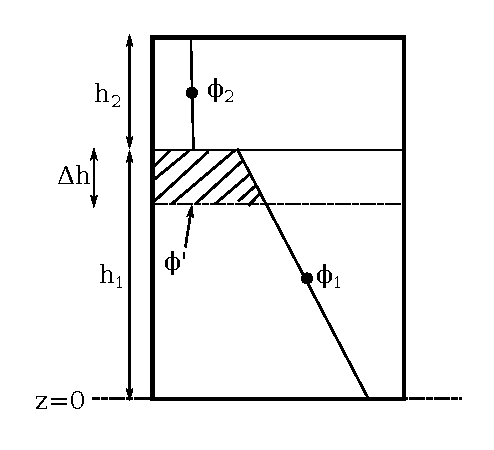
\includegraphics{../plots/schematic.pdf}
  \caption{\label{fig:schematic} A schematic demonstrating the ability for regridding/remapping to cause a decrease in RPE}
\end{figure}

\Cref{fig:schematic} shows a simple two-cell domain under regridding/remapping. The bottom cell has a mean tracer concentration of $\phi_1$ and thickness $h_1$. Similarly, the top cell has a mean tracer concentration of $\phi_2$ and thickness $h_2$. Regridding moves the interface between the cells from its initial position at $z = h_1$ to the dashed line at $z = h_1 - \Delta h$, and remapping mixes the integrated quantity of tracer $\phi'$ from the bottom cell to the top cell. Initially, the potential energy of the domain is

\begin{equation}
  PE_i = \frac{\phi_1 h_1 h_1}{2} + \phi_2 h_2\left(h_1 + \frac{h_2}{2}\right).
\end{equation}

After remapping, the potential energy becomes

\begin{equation}
  \begin{split}
    PE_f &= \left(\phi_1 h_1 - \phi'\right)\frac{h_1 - \Delta h}{2} \\
    &+ \left(\phi_2 h_2 + \phi'\right)\left(h_1 - \Delta h + \frac{h_2 + \Delta h}{2}\right).
  \end{split}
\end{equation}

Taking the difference between the final and initial potential energy gives the RPE change due to regridding/remapping,

\begin{equation}
  PE_f - PE_i = \frac{\phi'\left(h_1 + h_2\right)}{2} - \frac{\Delta h\left(\phi_1 h_1 + \phi_2 h_2\right)}{2}.
\end{equation}

With the condition that $\phi_1 > \phi_2$, it is possible for $PE_f - PE_i < 0$ when the remapping is higher order than piecewise constant (PCM). PCM is the lowest order reconstruction, and gives $\phi' = \phi_1 \Delta h$, thus $PE_f - PE_i \ge 0$.
